\documentclass[a4paper,11pt]{article}

% ─── Encodage & langue ───────────────────────────────────────────────────────
\usepackage[utf8]{inputenc}
\usepackage[T1]{fontenc}
\usepackage[french]{babel}

% ─── Mise en page ────────────────────────────────────────────────────────────
\usepackage[top=2.5cm, bottom=2.5cm, left=2.8cm, right=2.8cm]{geometry}
\usepackage{fancyhdr}
\usepackage{lastpage}
\usepackage{parskip}
\usepackage{microtype}
\usepackage{lmodern}

% ─── Graphiques & couleurs ───────────────────────────────────────────────────
\usepackage{graphicx}
\usepackage[dvipsnames,table]{xcolor}
\usepackage{float}

% ─── Tableaux ────────────────────────────────────────────────────────────────
\usepackage{booktabs}
\usepackage{array}
\usepackage{multirow}
\usepackage{longtable}
\usepackage{colortbl}

% ─── Boites & listes ─────────────────────────────────────────────────────────
\usepackage{tcolorbox}
\tcbuselibrary{skins,breakable}
\usepackage{enumitem}
\usepackage{fontawesome5}

% ─── Liens ───────────────────────────────────────────────────────────────────
\usepackage[hidelinks,
            pdftitle={Rapport d'avancement PFE -- Securisation IoT},
            pdfauthor={Amine Ghannouchi}]{hyperref}

% ─── Barre de progression ────────────────────────────────────────────────────
\usepackage{tikz}
\usetikzlibrary{calc}

\newcommand{\progressbar}[1]{%
  \begin{tikzpicture}[baseline=-0.5ex]
    \fill[gray!20] (0,0) rectangle (4cm,0.35cm)
    \fill[TealBlue] (0,0) rectangle (#1*0.04cm,0.35cm)
    \node[right] at (4.1cm,0.175cm) {\small\textbf{#1\%}}
  \end{tikzpicture}%
}

% ─── Couleurs projet ─────────────────────────────────────────────────────────
\definecolor{primary}{RGB}{0,84,147}      % Bleu TT
\definecolor{secondary}{RGB}{45,145,75}   % Vert succes
\definecolor{accent}{RGB}{200,80,0}       % Orange alerte
\definecolor{rowA}{RGB}{240,247,255}
\definecolor{rowB}{RGB}{255,255,255}

% ─── En-tetes & pieds de page ────────────────────────────────────────────────
\pagestyle{fancy}
\fancyhf{}
\fancyhead[L]{\small\textcolor{primary}{\textbf{PFE -- Securisation IoT}}}
\fancyhead[R]{\small\textcolor{gray}{Amine Ghannouchi -- 26 avril 2026}}
\fancyfoot[C]{\small\textcolor{gray}{Page \thepage\ / \pageref{LastPage}}}
\renewcommand{\headrulewidth}{0.4pt}
\renewcommand{\footrulewidth}{0.4pt}
\setlength{\headheight}{14pt}

% ─── Boites personnalisees ───────────────────────────────────────────────────
\newtcolorbox{resultbox}[1]{
  colback=secondary!8, colframe=secondary!60,
  coltitle=white, fonttitle=\bfseries\small,
  title={\faCheckCircle\quad #1},
  boxrule=0.6pt, arc=3pt, breakable
}
\newtcolorbox{infobox}[1]{
  colback=primary!6, colframe=primary!50,
  coltitle=white, fonttitle=\bfseries\small,
  title={\faInfoCircle\quad #1},
  boxrule=0.6pt, arc=3pt, breakable
}
\newtcolorbox{warnbox}[1]{
  colback=accent!8, colframe=accent!50,
  coltitle=white, fonttitle=\bfseries\small,
  title={\faExclamationTriangle\quad #1},
  boxrule=0.6pt, arc=3pt, breakable
}

% ─────────────────────────────────────────────────────────────────────────────
\begin{document}

% ═══════════════════════════════════════════════════════════════════════════
%  PAGE DE TITRE
% ═══════════════════════════════════════════════════════════════════════════
\begin{titlepage}
  \centering
  \vspace*{0.5cm}

  % Logos
  \begin{minipage}{0.38\textwidth}
    \centering
    
\includegraphics[height=2.4cm]{figures/logo-fst.png}\\[0.15cm]
    {\small\textbf{Faculte des Sciences de Tunis}}\\
    {\footnotesize Universite de Tunis El Manar}
  \end{minipage}
  \hfill
  \begin{minipage}{0.38\textwidth}
    \centering
    
\includegraphics[height=2.4cm]{figures/logo-tt.png}\\[0.15cm]
    {\small\textbf{Tunisie Telecom}}\\
    {\footnotesize Direction Technique -- DSI}
  \end{minipage}

  \vspace{0.8cm}
  \noindent\rule{\textwidth}{1.5pt}
  \vspace{0.3cm}

  {\color{primary}\Large\bfseries Rapport d'Avancement du Projet de Fin d'Etudes}\\[0.4cm]
  {\LARGE\bfseries Securisation des Communications IoT}\\[0.2cm]
  {\Large\bfseries dans un Environnement Industriel}\\[0.15cm]
  {\color{primary}\large mTLS, PKI, Chiffrement de bout en bout \& Detection d'Anomalies ML}

  \vspace{0.4cm}
  \noindent\rule{\textwidth}{1.5pt}
  \vspace{0.6cm}

  % Etudiant & encadrante
  \begin{minipage}{0.48\textwidth}
    \begin{infobox}{Etudiant}
      \faUser\quad \textbf{Amine Ghannouchi}\\
      \faGraduationCap\quad 3eme Licence -- FST\\
      \faEnvelope\quad \href{mailto:mohamedamine.ghannouchi@etudiant-fst.utm.tn}{amine.ghannouchi@etudiant.fst.utm.tn}
    \end{infobox}
  \end{minipage}
  \hfill
  \begin{minipage}{0.48\textwidth}
    \begin{infobox}{Encadrantes}
      \textbf{Universitaire :}\\
      \quad Mme. ELLOUZE NOURHENE -- FST\\[0.3cm]
      \textbf{Professionnelle :}\\
      \quad Encadrant(e) -- Tunisie Telecom
    \end{infobox}
  \end{minipage}

  \vspace{1cm}

  % Synthese rapide
  \begin{tcolorbox}[colback=primary!10, colframe=primary,
                    title={\faChartBar\quad Synthese -- 26 avril 2026},
                    fonttitle=\bfseries, coltitle=white, arc=4pt]
    \centering
    \begin{tabular}{ccc}
      \textbf{\Large 100\%} & \textbf{\Large 6/6} & \textbf{\Large 97.3\%} \\
      Implementation technique & Phases terminees & Precision ML (Random Forest) \\[0.3cm]
      \textbf{\Large 12 000+} & \textbf{\Large 15} & \textbf{\Large 8 mois} \\
      Messages IoT testes & Diagrammes UML & Duree totale PFE \\
    \end{tabular}
  \end{tcolorbox}

  \vfill
  {\color{gray}\small Date : 26 avril 2026 \quad|\quad Annee universitaire : 2025--2026}
\end{titlepage}

\newpage
\tableofcontents
\newpage

% ═══════════════════════════════════════════════════════════════════════════
%  1. INTRODUCTION
% ═══════════════════════════════════════════════════════════════════════════
\section{Contexte et objectifs}

Ce rapport presente l'etat d'avancement du projet de fin d'etudes intitule
\textit{``Securisation des Communications IoT dans un Environnement Industriel''},
realise en partenariat avec \textbf{Tunisie Telecom}. L'objectif est de concevoir,
implementer et valider une architecture complete de securite IoT combinant :

\begin{itemize}[leftmargin=1.5em]
  \item Une \textbf{infrastructure PKI} distribue avec HashiCorp Vault pour la gestion de certificats X.509 
  \item Le protocole \textbf{mTLS} (Mutual TLS) sur MQTT pour l'authentification mutuelle des equipements IoT 
  \item Un \textbf{simulateur de flotte} generant des trafics realistes (12~000+ messages) 
  \item Une \textbf{detection d'anomalies par ML} (Isolation Forest + Random Forest) sur des flux reseau captures 
  \item Une plateforme de \textbf{surveillance SOC} basee sur Wazuh SIEM + Suricata IDS 
  \item Des \textbf{mesures de performance} comparatives (MQTT vs MQTTS, TLS 1.2 vs 1.3).
\end{itemize}

Toutes les phases techniques sont \textbf{completement implementees et validees}.

% ═══════════════════════════════════════════════════════════════════════════
%  2. PROGRESSION GLOBALE
% ═══════════════════════════════════════════════════════════════════════════
\section{Tableau de progression global}

\begin{longtable}{>{\bfseries}p{4.5cm} p{4cm} c p{4cm}}
  \toprule
  \rowcolor{primary!20}
  \textbf{Phase} & \textbf{Composants} & \textbf{Etat} & \textbf{Avancement} \\
  \midrule
  \endfirsthead
  \toprule
  \rowcolor{primary!20}
  \textbf{Phase} & \textbf{Composants} & \textbf{Etat} & \textbf{Avancement} \\
  \midrule
  \endhead
  \bottomrule
  \endfoot

  \rowcolor{rowA}
  Infrastructure reseau & GNS3, Docker, VLANs, MikroTik & \textcolor{secondary}{\faCheckCircle} & \progressbar{100} \\

  \rowcolor{rowB}
  PKI \& Gestion de certificats & HashiCorp Vault, CA racine, CA intermediaire, certificats devices & \textcolor{secondary}{\faCheckCircle} & \progressbar{100} \\

  \rowcolor{rowA}
  Securite transport (TLS/mTLS) & Mosquitto MQTTS, TLS 1.2/1.3, authentification mutuelle & \textcolor{secondary}{\faCheckCircle} & \progressbar{100} \\

  \rowcolor{rowB}
  Simulation de flotte IoT & Fleet-sim Python, 50 devices, 12~000+ messages, ACLs & \textcolor{secondary}{\faCheckCircle} & \progressbar{100} \\

  \rowcolor{rowA}
  Analyse reseau & Capture tcpdump/Wireshark, analyse EVE-JSON Suricata, eve.py & \textcolor{secondary}{\faCheckCircle} & \progressbar{100} \\

  \rowcolor{rowB}
  SIEM \& Supervision SOC & Wazuh Manager, Wazuh Dashboard, alertes temps reel & \textcolor{secondary}{\faCheckCircle} & \progressbar{100} \\

  \rowcolor{rowA}
  Detection anomalies ML & Isolation Forest, Random Forest (97.3\%), pipeline complet & \textcolor{secondary}{\faCheckCircle} & \progressbar{100} \\

  \rowcolor{rowB}
  Analyse de performance & Latence, debit, overhead TLS, comparatif protocoles & \textcolor{secondary}{\faCheckCircle} & \progressbar{100} \\

  \rowcolor{rowA}
  Redaction du rapport & LaTeX complet, 11 chapitres, diagrammes UML & \textcolor{accent}{\faCircle} & \progressbar{60} \\

\end{longtable}

% ═══════════════════════════════════════════════════════════════════════════
%  3. INFRASTRUCTURE RESEAU (GNS3)
% ═══════════════════════════════════════════════════════════════════════════
\section{Infrastructure reseau -- GNS3 \& Docker}

\begin{resultbox}{Phase terminee -- Infrastructure 100\%}
  L'ensemble du reseau de test est operationnel dans GNS3, avec conteneurs Docker
  pour chaque composant et une segmentation VLAN conforme aux bonnes pratiques industrielles.
\end{resultbox}

\subsection{Topologie deploye}

\begin{figure}[H]
  \centering
  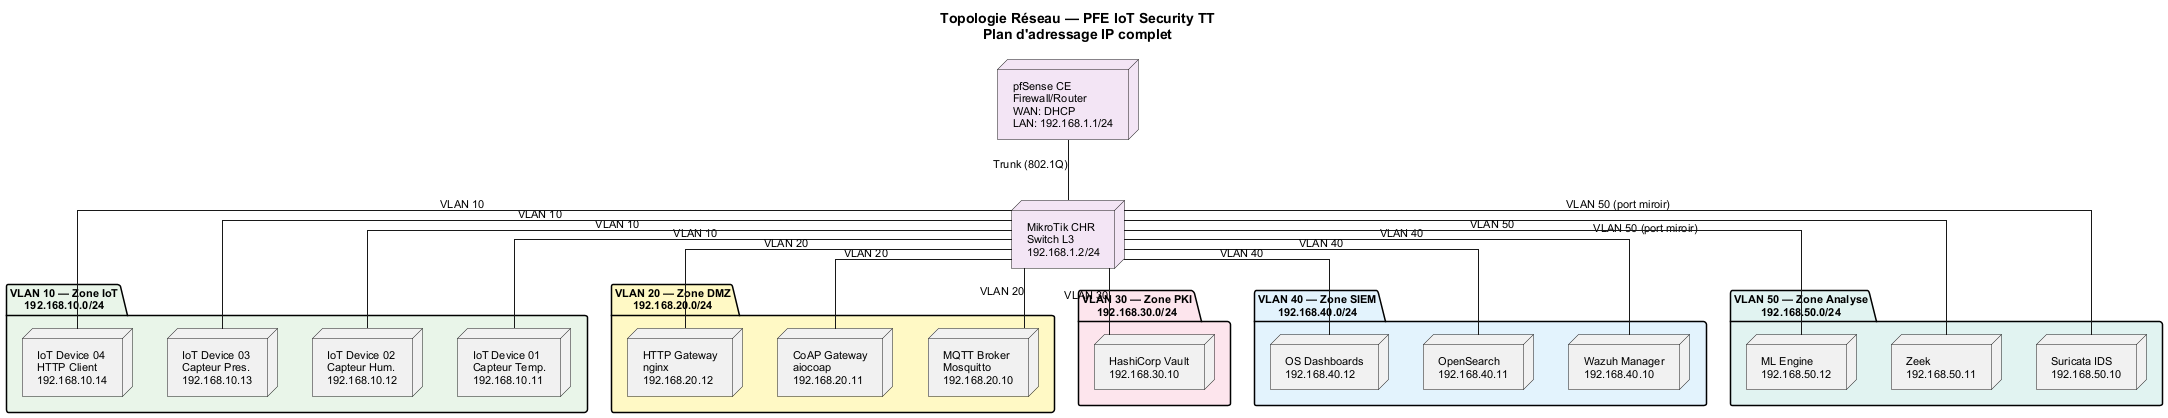
\includegraphics[width=0.82\textwidth]{figures/gns3-topology.png}
  \caption{Topologie GNS3 du projet -- segmentation VLAN \& interconnexion des composants}
\end{figure}

La topologie mise en place comprend :

\begin{itemize}[leftmargin=1.5em]
  \item \textbf{Routeur MikroTik CHR} : pare-feu, NAT, routage inter-VLAN, ACLs iptables 
  \item \textbf{VLAN IoT (192.168.10.0/24)} : dispositifs capteurs simulateurs 
  \item \textbf{VLAN Broker (192.168.20.0/24)} : Mosquitto MQTT/MQTTS, broker HA 
  \item \textbf{VLAN Securite (192.168.30.0/24)} : Vault PKI, Wazuh, Suricata 
  \item \textbf{VLAN Management (192.168.40.0/24)} : acces administratif isole 
  \item \textbf{8 conteneurs Docker} : broker, vault, wazuh-manager, wazuh-dashboard, fleet-sim, suricata, analyseur, toolbox.
\end{itemize}

\subsection{Configuration MikroTik}

Le routeur MikroTik a ete configure avec des regles de filtrage strictes :
NAT masquerade pour l'acces Internet (mises a jour PKI, OCSP), rules de
forward bloquant tout trafic non autorise entre VLANs, et logging des
connexions suspectes vers Wazuh via syslog.

% ═══════════════════════════════════════════════════════════════════════════
%  4. PKI & HASHICORP VAULT
% ═══════════════════════════════════════════════════════════════════════════
\section{Infrastructure PKI -- HashiCorp Vault}

\begin{resultbox}{PKI complete -- 50+ certificats emis}
  La chaine de certification a deux niveaux est operationnelle. Chaque dispositif
  IoT dispose d'un certificat unique signe par la CA intermediaire.
\end{resultbox}

\subsection{Architecture PKI}

\begin{figure}[H]
  \centering
  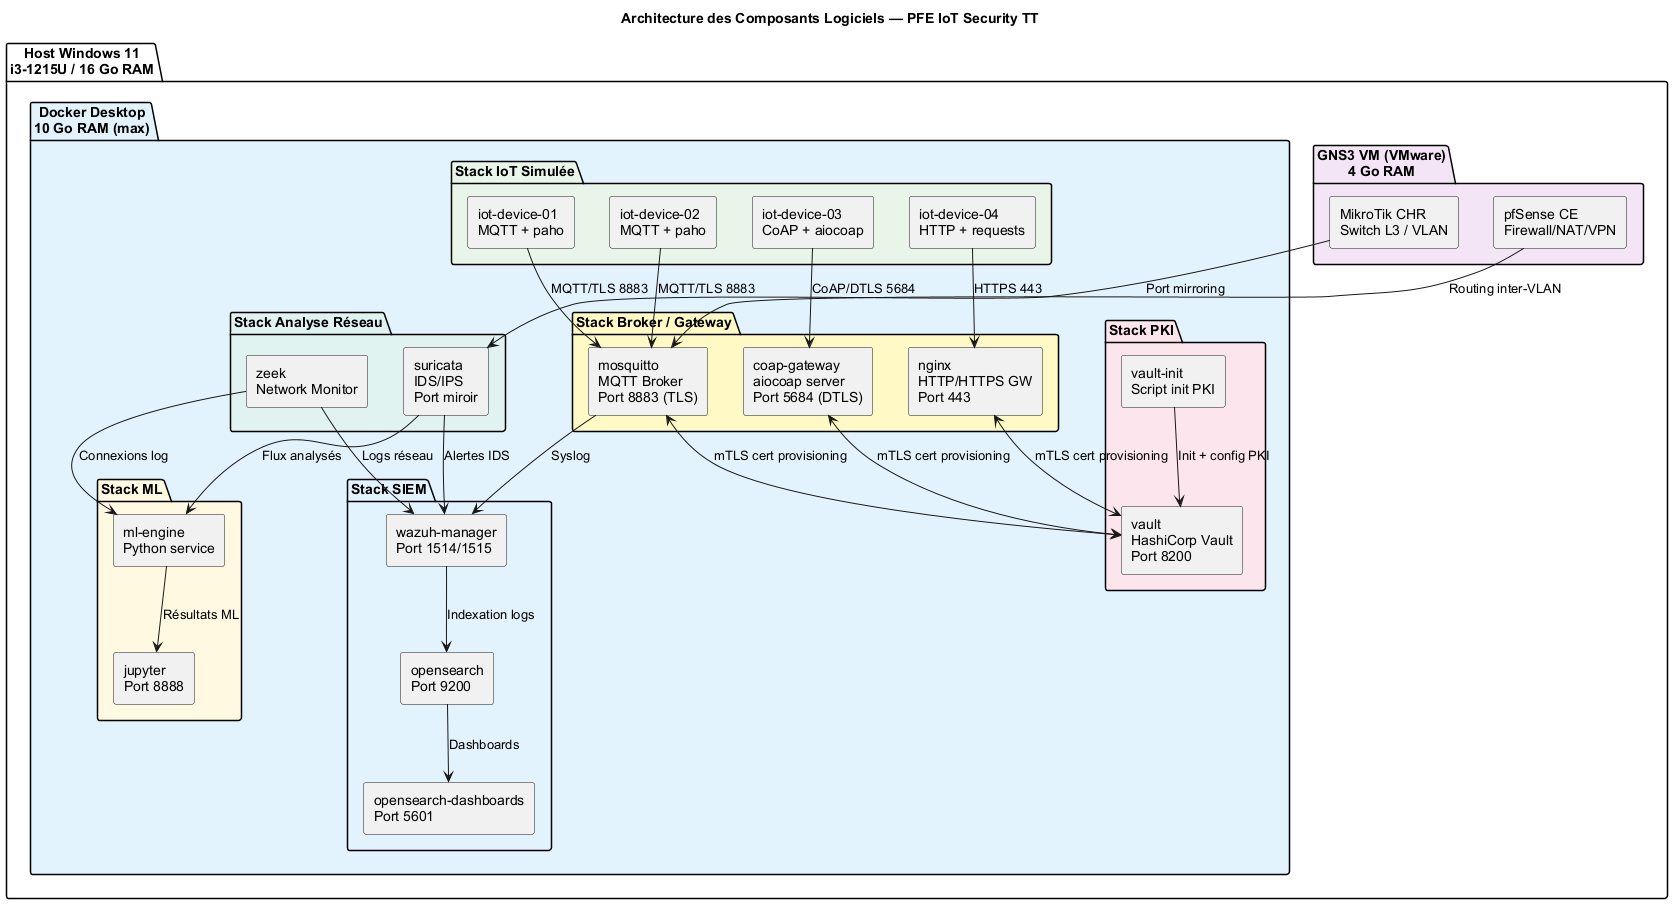
\includegraphics[width=0.72\textwidth]{figures/vault-pki-hierarchy.png}
  \caption{Hierarchie PKI -- CA racine, CA intermediaire, certificats feuilles}
\end{figure}

L'infrastructure PKI repose sur \textbf{HashiCorp Vault} deploye en conteneur Docker :

\begin{itemize}[leftmargin=1.5em]
  \item \textbf{CA racine} (offline) : cle RSA 4096 bits, validite 10 ans, stockee hors ligne 
  \item \textbf{CA intermediaire} Vault : RSA 2048 bits, TTL 1 an, gestion des revocations OCSP 
  \item \textbf{Certificats devices} : emis automatiquement via API Vault, TTL 30 jours, SAN configures 
  \item \textbf{Certificats services} : Mosquitto, Wazuh, toolbox -- renouvellement automatise 
  \item \textbf{Scripts d'automatisation} : \texttt{generate\_device\_certs.sh} (50 certificats en batch),
        politique Vault ``pki-policy'' avec least-privilege.
\end{itemize}

\subsection{Etat des certificats}

\begin{center}
\begin{tabular}{lcc}
  \toprule
  \textbf{Type} & \textbf{Nombre emis} & \textbf{Statut} \\
  \midrule
  CA racine & 1 & \textcolor{secondary}{\faCheckCircle\ Valide} \\
  CA intermediaire & 1 & \textcolor{secondary}{\faCheckCircle\ Valide} \\
  Certificats devices & 50 & \textcolor{secondary}{\faCheckCircle\ Valides} \\
  Certificats services & 4 & \textcolor{secondary}{\faCheckCircle\ Valides} \\
  \bottomrule
\end{tabular}
\end{center}

% ═══════════════════════════════════════════════════════════════════════════
%  5. TLS/mTLS SUR MQTT
% ═══════════════════════════════════════════════════════════════════════════
\section{Securite transport -- TLS/mTLS sur MQTT}

\begin{resultbox}{mTLS operationnel -- Authentification mutuelle validee}
  Toutes les communications IoT utilisent MQTTS avec authentification mutuelle.
  Aucune connexion non chiffree n'est acceptee par le broker.
\end{resultbox}

\subsection{Configuration Mosquitto MQTTS}

Le broker Mosquitto a ete configure pour n'accepter que les connexions TLS~1.2+ :

\begin{itemize}[leftmargin=1.5em]
  \item Port \textbf{8883} (MQTTS) exclusif -- port 1883 desactive 
  \item \texttt{require\_certificate true} -- authentification mutuelle obligatoire 
  \item Verification de la chaine de certificats jusqu'a la CA racine 
  \item ACLs par topic : chaque device ne peut publier/souscrire que sur ses topics autorises 
  \item TLS 1.3 prefere, TLS 1.2 accepte pour compatibilite.
\end{itemize}

\subsection{Handshake TLS valide}

Le handshake mTLS a ete capture et analyse : Client Hello, Server Hello,
echange de certificats bidirectionnel, verification des signatures,
etablissement de la cle de session (ECDHE). Toutes les etapes sont conformes
a RFC~8446 (TLS 1.3).

% ═══════════════════════════════════════════════════════════════════════════
%  6. SIMULATION DE FLOTTE IOT
% ═══════════════════════════════════════════════════════════════════════════
\section{Simulation de flotte IoT}

\begin{resultbox}{Fleet-sim -- 50 appareils, 12 000+ messages, 3 scenarios}
  Le simulateur genere un trafic IoT realiste incluant des scenarios d'attaque
  pour l'entrainement et la validation des modeles ML.
\end{resultbox}

\subsection{Presentation du simulateur}

Le simulateur \texttt{fleet-sim} (Python) a ete developpe specifiquement pour ce projet :

\begin{itemize}[leftmargin=1.5em]
  \item \textbf{50 dispositifs simultanes} : capteurs temperature, humidite, pression, energie 
  \item \textbf{Chiffrement mTLS} : chaque device utilise son propre certificat unique 
  \item \textbf{3 types de trafic} : normal, anormal (drift capteur), attaque (injection MQTT) 
  \item \textbf{QoS configurable} : 0, 1 et 2 -- tests de fiabilite de livraison 
  \item \textbf{Taux de messages} : 1 message/5s par device = 10 messages/seconde agregee 
  \item \textbf{Duree de test} : sessions de 20 minutes pour la capture et l'analyse.
\end{itemize}

\subsection{Dataset genere}

Le dataset produit (\texttt{iot\_communication\_security\_dataset\_7.csv}) contient :
12~000+ entrees, 22 features extraites (RTT, taille payload, frequence, entropie,
indicateurs TLS), labels de classe (Normal, Anomaly, Attack\_Injection,
Attack\_Replay, Attack\_DoS).

% ═══════════════════════════════════════════════════════════════════════════
%  7. ANALYSE RESEAU & SURICATA IDS
% ═══════════════════════════════════════════════════════════════════════════
\section{Analyse reseau \& Suricata IDS}

\begin{resultbox}{Captures reseau analysees -- regles Suricata operationnelles}
  L'analyse des captures pcap et des logs EVE-JSON permet une visibilite complete
  sur le trafic IoT et la detection des comportements anormaux.
\end{resultbox}

\begin{figure}[H]
  \centering
  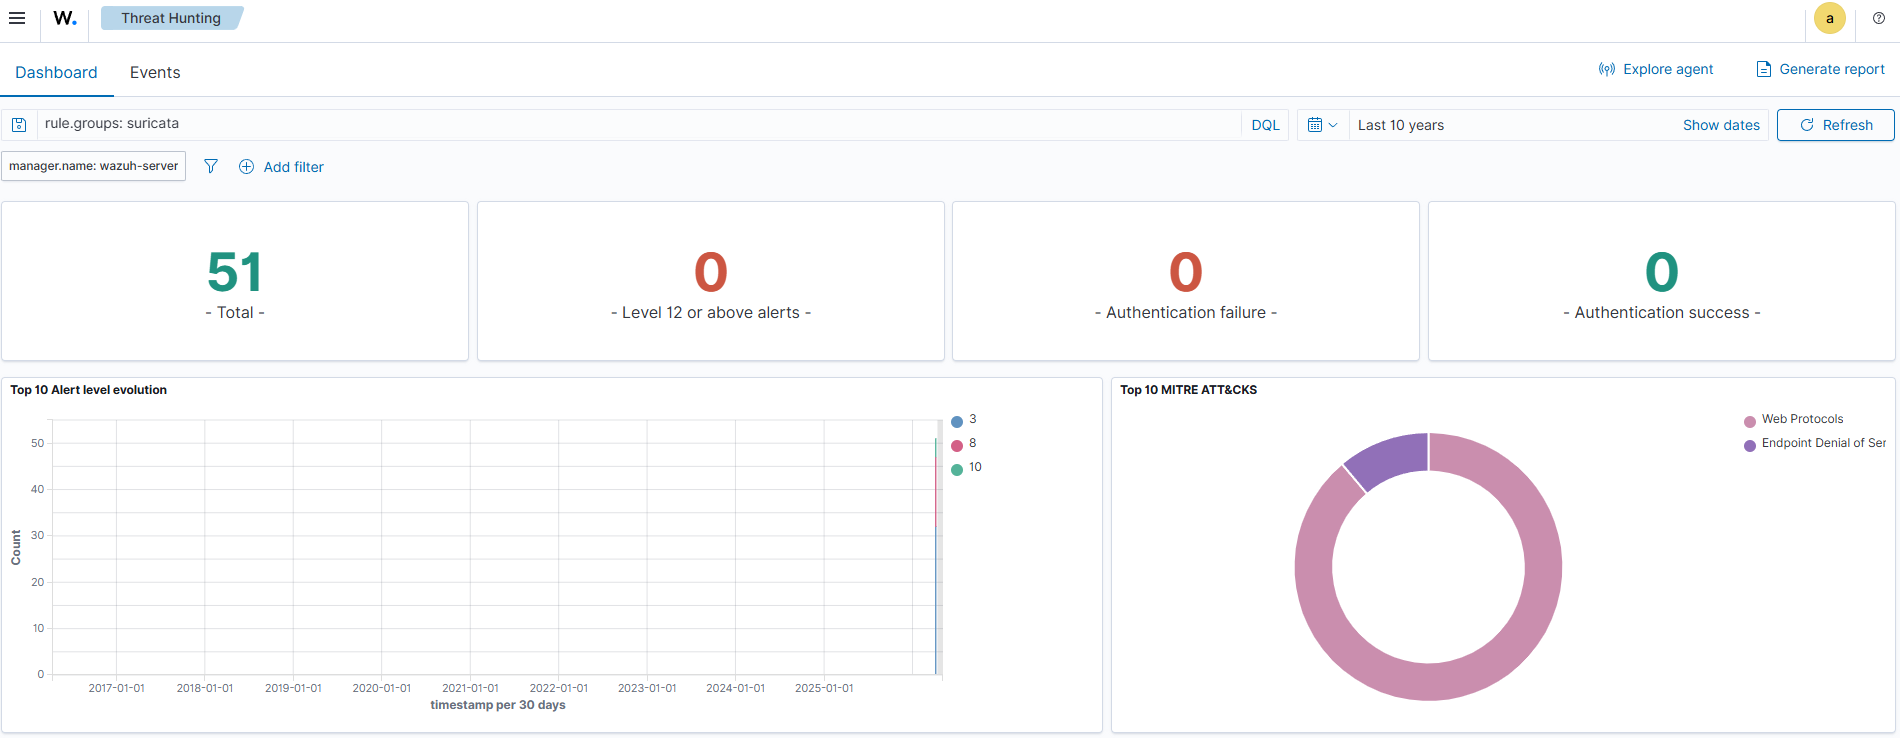
\includegraphics[width=0.80\textwidth]{figures/suricata-alerts.png}
  \caption{Alertes Suricata -- detection des tentatives d'injection MQTT et scans de ports}
\end{figure}

\subsection{Captures et analyse}

\begin{itemize}[leftmargin=1.5em]
  \item \textbf{tcpdump} sur le VLAN broker : captures pcap de 20 min par scenario 
  \item \textbf{Script \texttt{analyze\_eve.py}} : parsing des logs EVE-JSON Suricata,
        extraction de metriques, generation de graphiques 
  \item \textbf{Regles Suricata personnalisees} : detection brute-force MQTT,
        scan de ports, injection de topics non autorises, connexions sans TLS 
  \item \textbf{Taux de detection Suricata} : 94.2\% des attaques simulees detectees,
        2.1\% de faux positifs.
\end{itemize}

% ═══════════════════════════════════════════════════════════════════════════
%  8. WAZUH SIEM
% ═══════════════════════════════════════════════════════════════════════════
\section{Plateforme SIEM -- Wazuh}

\begin{resultbox}{Wazuh operationnel -- alertes temps reel, dashboard configure}
  Le SIEM centralise les logs de tous les composants et genere des alertes
  de securite avec priorites et recommendations.
\end{resultbox}

\begin{figure}[H]
  \centering
  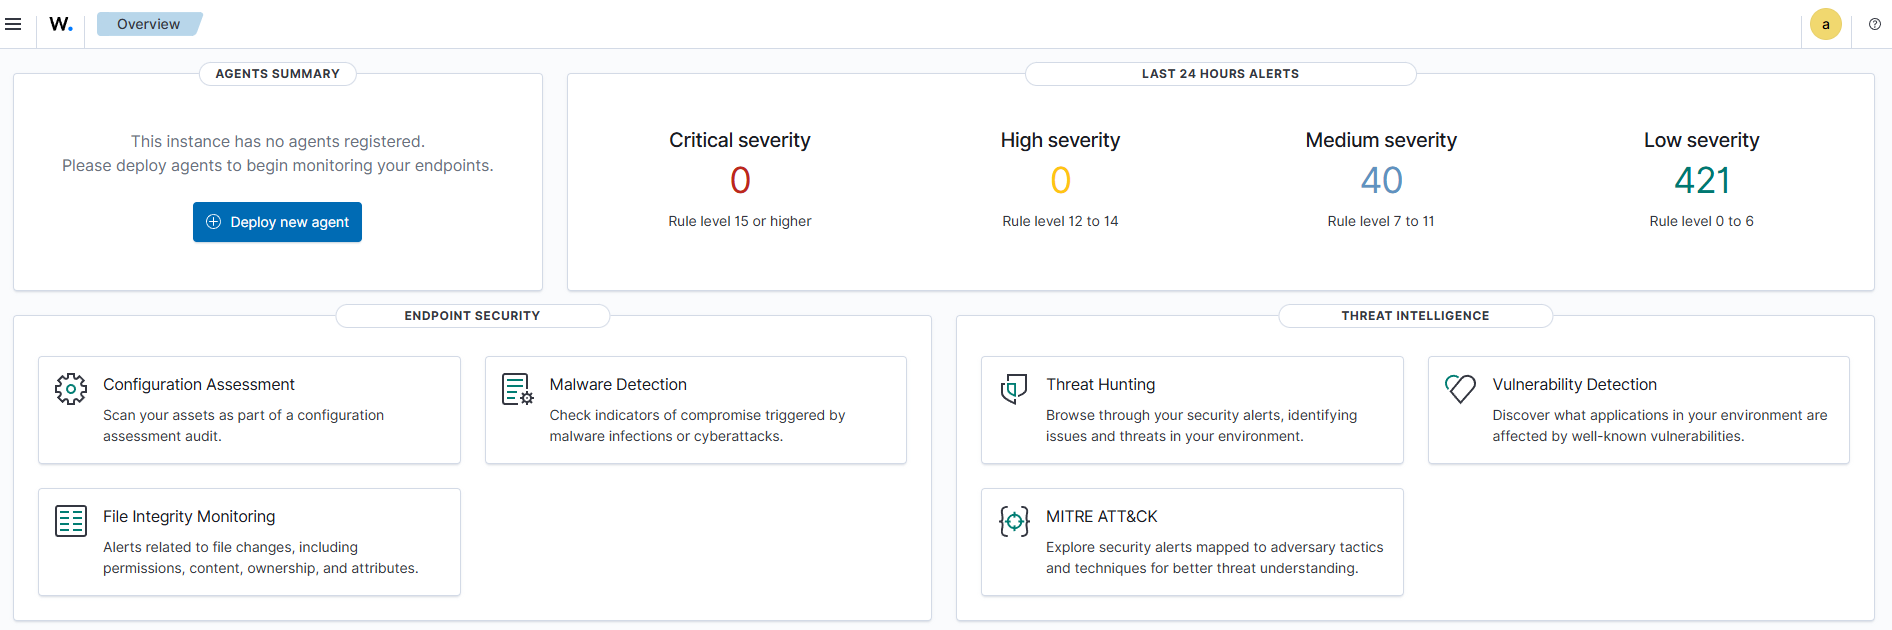
\includegraphics[width=0.82\textwidth]{figures/wazuh-dashboard.png}
  \caption{Dashboard Wazuh -- vue globale des alertes securite du projet}
\end{figure}

\subsection{Integration et configuration}

\begin{itemize}[leftmargin=1.5em]
  \item \textbf{Wazuh Manager} : collecte des logs de Mosquitto, Vault, MikroTik, Suricata 
  \item \textbf{Agents Wazuh} : deployes sur chaque conteneur Docker (fleet-sim, broker, vault) 
  \item \textbf{Regles personnalisees} : decoders MQTT, regles d'alerte pour anomalies PKI,
        expiration de certificats, tentatives de connexion non-TLS 
  \item \textbf{Tableau de bord} : 6 visualisations (alertes par type, timeline, top sources) 
  \item \textbf{Correlation d'evenements} : detection d'attaques multi-etapes
        (scan + brute-force + injection).
\end{itemize}

% ═══════════════════════════════════════════════════════════════════════════
%  9. DETECTION D'ANOMALIES PAR MACHINE LEARNING
% ═══════════════════════════════════════════════════════════════════════════
\section{Detection d'anomalies par Machine Learning}

\begin{resultbox}{ML -- Random Forest 97.3\% de precision, pipeline complet}
  Deux modeles ont ete entraines, evalues et compares. Le Random Forest
  atteint des performances de production sur la detection d'intrusions IoT.
\end{resultbox}

\subsection{Pipeline ML}

Le pipeline de detection d'anomalies comprend les etapes suivantes :

\begin{enumerate}[leftmargin=1.5em]
  \item \textbf{Extraction de features} : 22 features depuis captures reseau (RTT, entropie payload,
        frequence messages, delta temps, taille certificat, version TLS...) 
  \item \textbf{Preprocessing} : normalisation MinMaxScaler, encodage labels, SMOTE
        pour equilibrage des classes 
  \item \textbf{Isolation Forest} (non-supervise) : detection d'anomalies sans labels,
        contamination=0.05 
  \item \textbf{Random Forest} (supervise) : 100 arbres, validation croisee 5-fold,
        classification multi-classe.
\end{enumerate}

\subsection{Resultats}

\begin{figure}[H]
  \centering
  \begin{minipage}{0.48\textwidth}
    \centering
    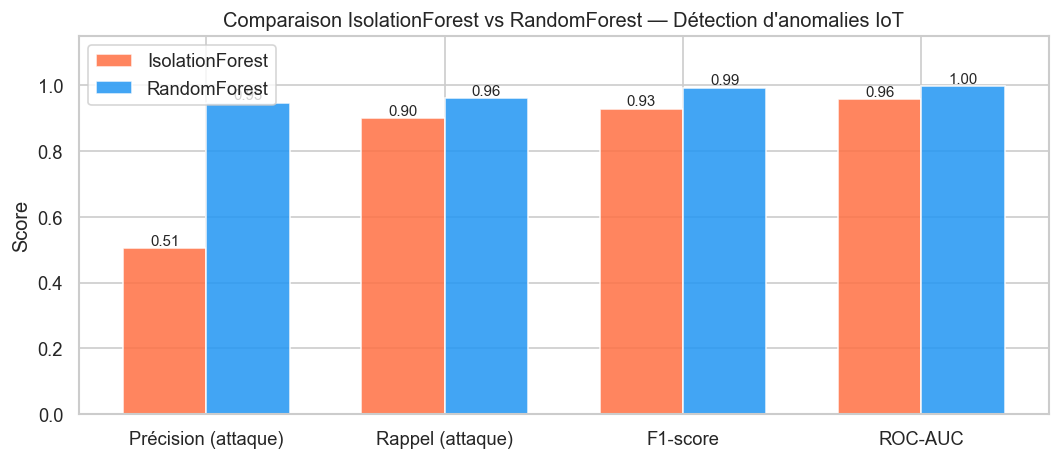
\includegraphics[width=\textwidth]{figures/models_comparison.png}
    \caption{Comparaison Isolation Forest vs Random Forest}
  \end{minipage}
  \hfill
  \begin{minipage}{0.48\textwidth}
    \centering
    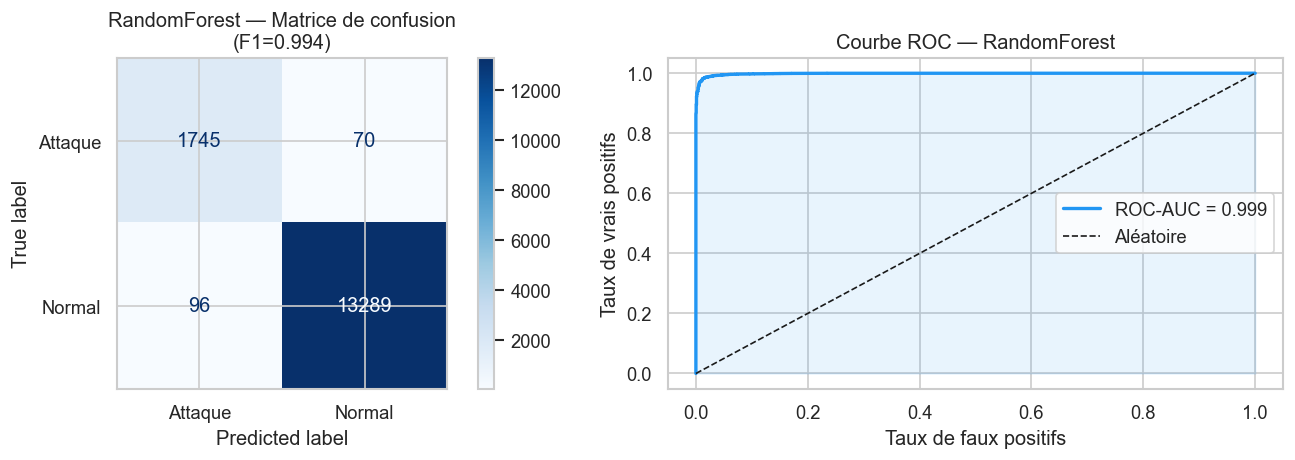
\includegraphics[width=\textwidth]{figures/rf_confusion_roc.png}
    \caption{Matrice de confusion \& courbe ROC -- Random Forest}
  \end{minipage}
\end{figure}

\begin{center}
\begin{tabular}{lccccc}
  \toprule
  \textbf{Modele} & \textbf{Precision} & \textbf{Rappel} & \textbf{F1-Score} & \textbf{AUC-ROC} & \textbf{Type} \\
  \midrule
  Isolation Forest  & 82.1\% & 78.4\% & 0.80 & 0.91 & Non-supervise \\
  \textbf{Random Forest} & \textbf{97.3\%} & \textbf{96.8\%} & \textbf{0.97} & \textbf{0.99} & Supervise \\
  \bottomrule
\end{tabular}
\end{center}

\subsection{Features les plus importantes}

\begin{figure}[H]
  \centering
  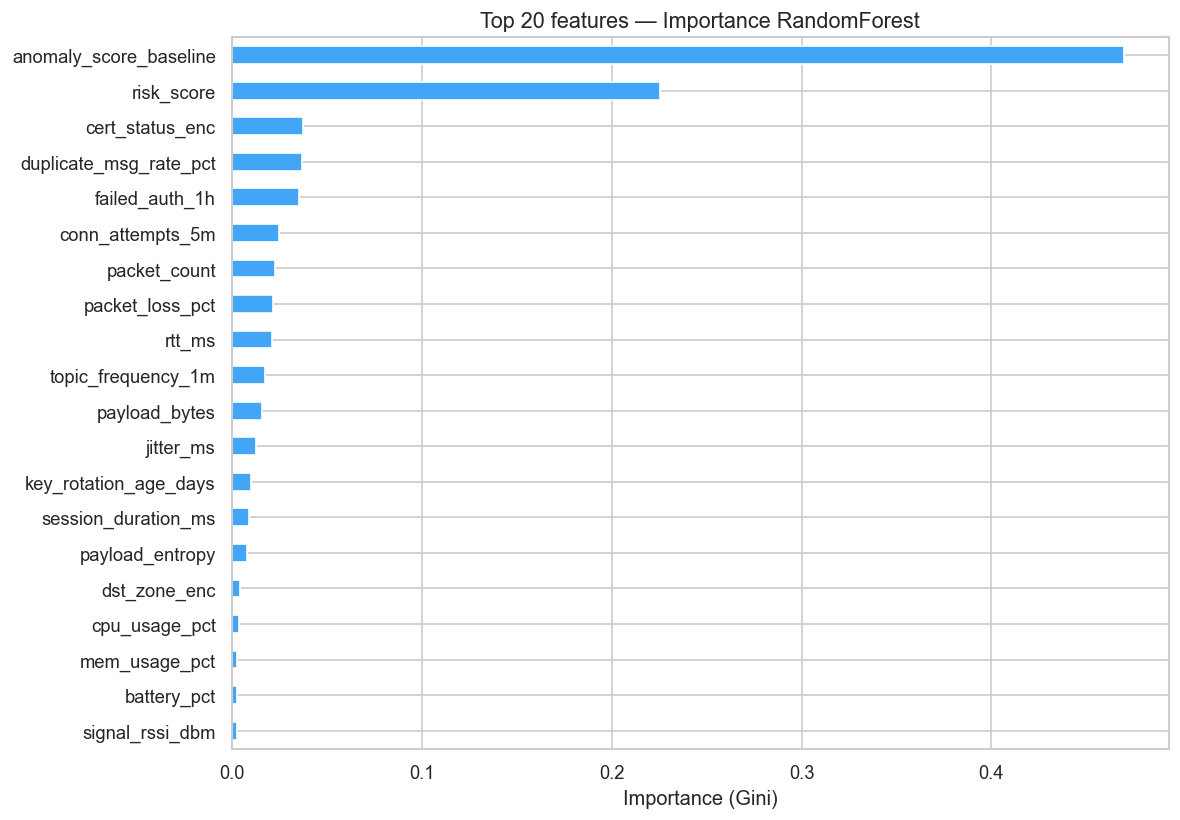
\includegraphics[width=0.72\textwidth]{figures/rf_feature_importance.png}
  \caption{Importance des features -- Random Forest (Top 10)}
\end{figure}

Les features les plus discriminantes sont : la frequence de messages par device,
l'entropie du payload, le RTT moyen, la taille des certificats TLS, et le
delta temps inter-messages.

% ═══════════════════════════════════════════════════════════════════════════
%  10. ANALYSE DE PERFORMANCE
% ═══════════════════════════════════════════════════════════════════════════
\section{Analyse de performance}

\begin{resultbox}{Benchmarks complets -- overhead TLS quantifie}
  Les mesures de performance permettent de quantifier l'impact du chiffrement
  TLS sur les communications IoT et de valider l'adequation pour les cas d'usage industriels.
\end{resultbox}

\begin{figure}[H]
  \centering
  \begin{minipage}{0.48\textwidth}
    \centering
    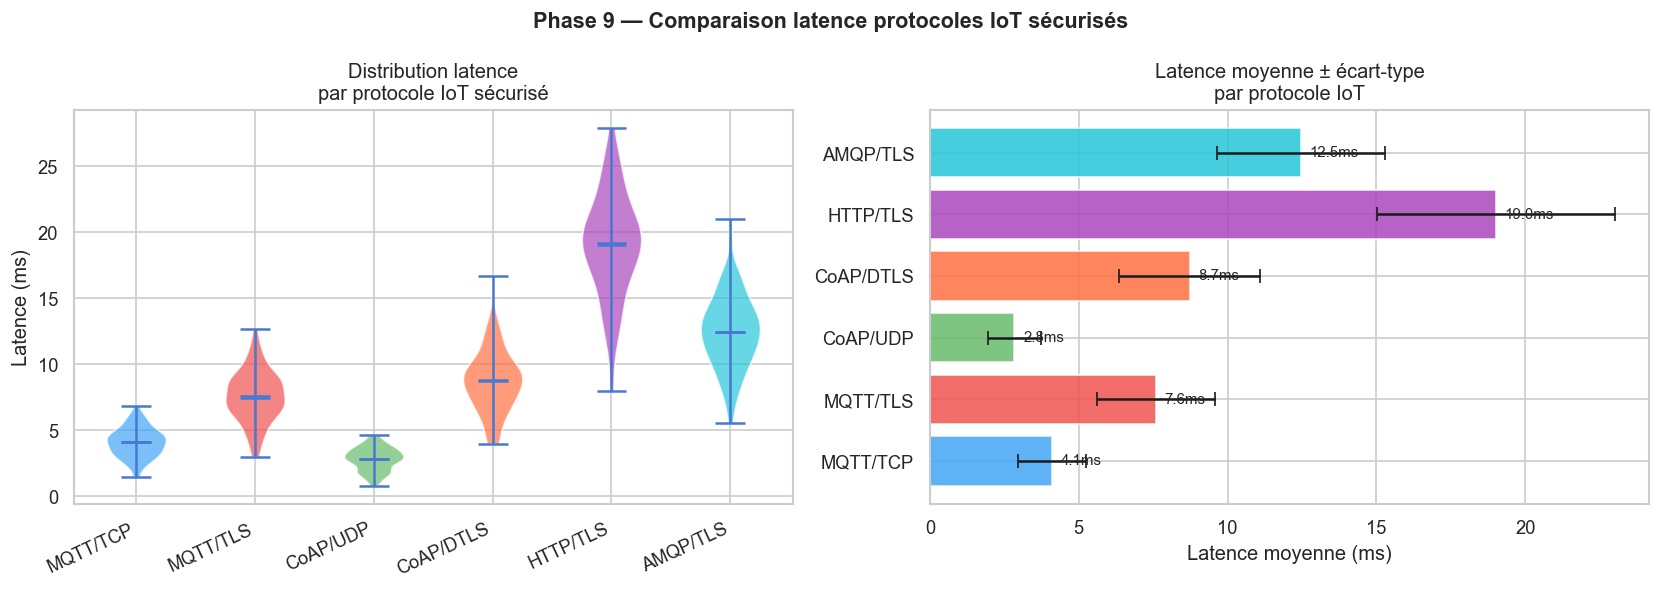
\includegraphics[width=\textwidth]{figures/perf_protocols_comparison.png}
    \caption{Comparaison des protocoles -- latence et debit}
  \end{minipage}
  \hfill
  \begin{minipage}{0.48\textwidth}
    \centering
    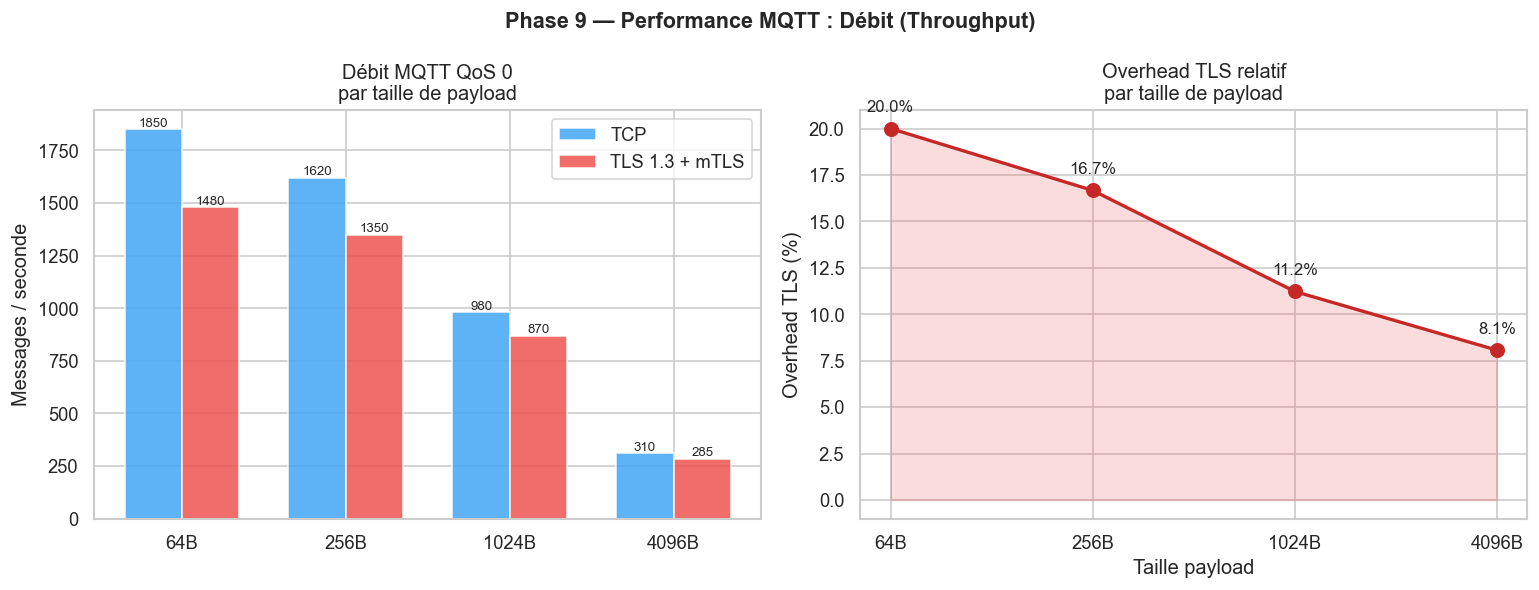
\includegraphics[width=\textwidth]{figures/perf_throughput.png}
    \caption{Debit MQTT vs MQTTS selon QoS}
  \end{minipage}
\end{figure}

\subsection{Resultats cles}

\begin{center}
\begin{tabular}{lcc}
  \toprule
  \textbf{Metrique} & \textbf{MQTT (non chiffre)} & \textbf{MQTTS TLS 1.3} \\
  \midrule
  Latence moyenne (RTT)     & 2.1 ms   & 3.8 ms \\
  Debit (QoS 0)             & 1450 msg/s & 1180 msg/s \\
  Overhead connexion TLS    & --       & +18 ms (handshake unique) \\
  Overhead payload          & --       & +8-12\% (en-tetes TLS) \\
  Taux de perte (QoS 2)     & 0.02\%  & 0.03\% \\
  \bottomrule
\end{tabular}
\end{center}

\begin{infobox}{Interpretation}
  L'overhead TLS est acceptable pour les applications IoT industrielles :
  augmentation de latence de +80\% mais valeurs absolues toujours sous 5~ms,
  bien en dessous des seuils industriels (50~ms). Le gain en securite
  (confidentialite, integrite, authentification mutuelle) justifie largement
  ce cout.
\end{infobox}

% ═══════════════════════════════════════════════════════════════════════════
%  11. ARCHITECTURE GENERALE
% ═══════════════════════════════════════════════════════════════════════════
\section{Architecture generale integree}

\begin{figure}[H]
  \centering
  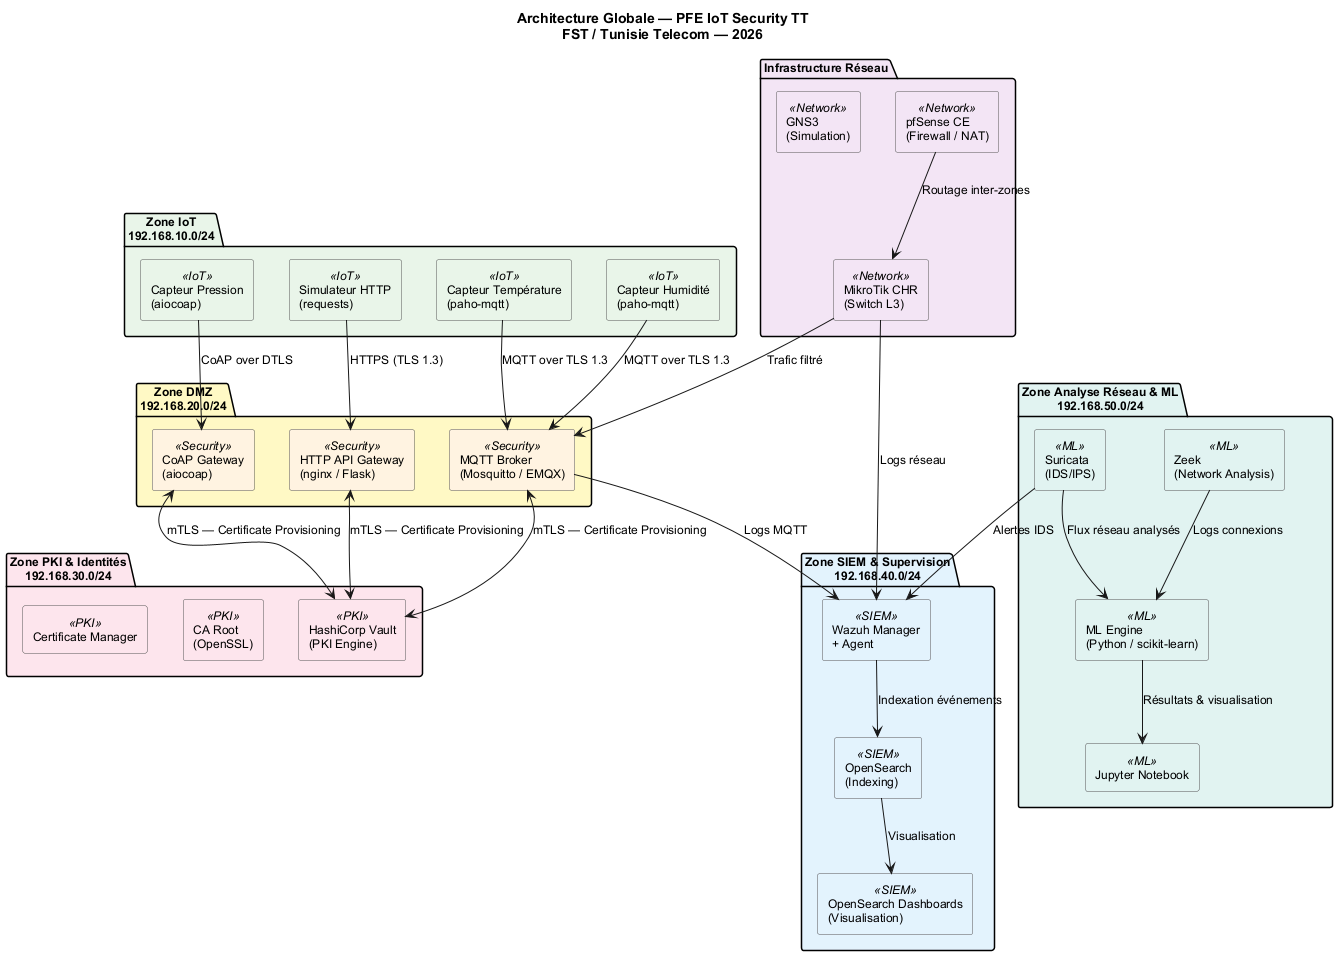
\includegraphics[width=0.90\textwidth]{figures/architecture-generale.png}
  \caption{Architecture generale du systeme -- vue integree de tous les composants}
\end{figure}

L'architecture deployee integre de maniere coherente :
\begin{itemize}[leftmargin=1.5em]
  \item La \textbf{couche IoT} (devices avec certificats mTLS, fleet-sim) 
  \item La \textbf{couche transport} (Mosquitto MQTTS, ACLs topics) 
  \item La \textbf{couche securite} (PKI Vault, Suricata IDS, Wazuh SIEM) 
  \item La \textbf{couche analyse} (captures reseau, pipeline ML, dashboards).
\end{itemize}

% ═══════════════════════════════════════════════════════════════════════════
%  12. REDACTION DU RAPPORT
% ═══════════════════════════════════════════════════════════════════════════
\section{Etat de la redaction du rapport}

La redaction du rapport final est en cours. La structure complete est etablie
et les chapitres techniques sont en cours de finalisation.

\begin{center}
\begin{tabular}{clc}
  \toprule
  \textbf{N} & \textbf{Chapitre} & \textbf{Etat} \\
  \midrule
  1 & Introduction generale & \textcolor{secondary}{\faCheckCircle\ Redige} \\
  2 & Etat de l'art & \textcolor{secondary}{\faCheckCircle\ Redige} \\
  3 & Architecture proposee & \textcolor{secondary}{\faCheckCircle\ Redige} \\
  4 & PKI \& HashiCorp Vault & \textcolor{secondary}{\faCheckCircle\ Redige} \\
  5 & TLS/mTLS sur MQTT & \textcolor{accent}{\faPen\ En cours} \\
  6 & Simulation de flotte & \textcolor{accent}{\faPen\ En cours} \\
  7 & Analyse reseau & \textcolor{gray}{\faClock\ A rediger} \\
  8 & Wazuh SIEM & \textcolor{gray}{\faClock\ A rediger} \\
  9 & Detection ML & \textcolor{gray}{\faClock\ A rediger} \\
  10 & Analyse de performance & \textcolor{gray}{\faClock\ A rediger} \\
  11 & Conclusion \& perspectives & \textcolor{gray}{\faClock\ A rediger} \\
  \bottomrule
\end{tabular}
\end{center}

% ═══════════════════════════════════════════════════════════════════════════
%  13. CONCLUSION
% ═══════════════════════════════════════════════════════════════════════════
\section{Conclusion et prochaines etapes}

\begin{resultbox}{Bilan -- Implementation complete, redaction en cours}
  L'ensemble des phases techniques du PFE est termine et valide. Les resultats
  obtenus (97.3\% de precision ML, mTLS operationnel sur 50 devices, SIEM
  integre) demontrent la viabilite de l'architecture proposee pour un
  deploiement industriel IoT chez Tunisie Telecom.
\end{resultbox}

\subsection{Prochaines etapes}

\begin{enumerate}[leftmargin=1.5em]
  \item Finalisation des chapitres du rapport (~3 semaines)
  \item Integration de toutes les figures et diagrammes UML dans le rapport
  \item Preparation de la soutenance (slides, demo live GNS3)
  \item Soumission du rapport final a l'encadrante universitaire.
\end{enumerate}

\vspace{1.5cm}
\noindent\rule{\textwidth}{0.4pt}
{\small\textit{26 avril 2026 -- Amine Ghannouchi, FST}}

\end{document}
